\documentclass{article}

\usepackage[left=15mm,top=25mm,bottom=15mm,right=15mm,headheight=15mm,headsep=10mm,footskip=10mm]{geometry}
% \usepackage{ngerman}
\usepackage{scrextend}
\usepackage[latin1]{inputenc}
\usepackage[T1]{fontenc}
\usepackage{helvet}
\renewcommand{\familydefault}{\sfdefault}
% \usepackage[printwatermark]{xwatermark}							   
\usepackage{ulem}
\usepackage{here}
\usepackage{amsthm}
\usepackage{gensymb}
\usepackage{fancyhdr}
\pagestyle{fancy} 
\usepackage{longtable}
\usepackage{hhline}
\usepackage[table]{xcolor}
\usepackage{amsfonts}
\usepackage{amssymb}
\usepackage{amsmath}
\usepackage{mathcomp}
\usepackage{tabularx}
% \newcolumntype{L}[1]{>{\raggedright\arraybackslash}p{#1}} % linksb�ndig mit Breitenangabe
\usepackage{multicol}
\usepackage{footnote}
\usepackage{multirow}
\usepackage{graphicx}
\usepackage{listings}
\usepackage{hyperref} 
\usepackage[final]{pdfpages}
\usepackage{floatflt,epsfig}
\usepackage[export]{adjustbox}
\usepackage{listings}
\usepackage[pdf]{graphviz}

% \newwatermark[allpages,color=gray!50,angle=45,scale=2.5,xpos=0,ypos=0]{for internal use only}

\rhead{\includegraphics[width=.3\textwidth,]{src/_recendt}}
\usepackage{enumitem}

\makesavenoteenv{tabular}
% \makesavenoteenv{table}
\definecolor{maroon}{cmyk}{0,0.87,0.68,0.32}


\lstdefinestyle{Codeschnipsel}{
language=C,
basicstyle=\sffamily\small,
keywordstyle={\color{blue}\bfseries},
%identifierstyle={\color{DarkRed}},
commentstyle={\color{green}\slshape},
stringstyle={\color{orange}},
backgroundcolor={\color{Cornsilk}},
%columns=fullflexible,
frame=shadowbox,
rulesepcolor=\color{green},
morekeywords={uint8_t, uint16_t, uint32_t, bool}, % eigene Keywörter
basewidth={0.4em,0.3em},
fontadjust=true,
breaklines=true,
showspaces=false,
showtabs=false
}


\newcommand{\lstC}{\lstinline[style=Codeschnipsel]}

\newcommand{\spec}[4]
	{\vspace{1mm}
			% \begin{table}[H]
			\begin{tabular}{|p{3cm}|p{15cm}|}
			\hline
		\redrow	\hline 	Tag #1		& \begin{tabular}{p{7.5cm}|l|l} #2 & Module & #3 \end{tabular} \\
				\hline Description				& #4 \\															
				\hline
			\end{tabular}
			% \label{#1}
		% \end{table}
	}
\newcommand{\TODO}[1]{\textcolor{red}{\textbf{ToDo:} #1}}
\newcommand{\redrow}{\rowcolor{red!70}}

% \newcommand{\ltab}{\raggedright\arraybackslash} % Tabellenabschnitt rechtsbündig
\newcommand{\req}[9]
{
		\begin{table}[H]
		\begin{tabular}{|p{3cm}|p{15cm}|}
		% \hline
	\redrow	\hline 	Tag #1		& \begin{tabular}{p{7.5cm}|l|l} #2 & Module & #9 \end{tabular} \\
			% \hline Priority				& \begin{tabular}{p{7.5cm}|l|l} #3 & Status & #4 \end{tabular}  \\		% (h)igh/(m)id/(l)ow
			\hline Description				& #5 \\															% todo/WIP/test/done
			% \hline Input				& \begin{tabular}{p{7.5cm}|l|l} #6 & Output & #8 \end{tabular} \\
			% \hline Operation			& #7 \\
			\hline
		\end{tabular}
		\label{#1}
	\end{table}
}
\newcommand{\sol}[1]{ \textbf{Solution for REQ\##1:} }


	% \req{ \# }{title}{ H/M/L }{ stat }
	% { desc }
	% { in }	{ op }	{ out }	{module}


	% \par
		% \begin{center}	\bf	\huge	OCT-IO-Board 'Octane'	\end{center}

% \include{src/_document_OCTaneFW}


\begin{document}
\pagestyle{empty} 
	\parindent0pt %Einr�cken bei neuer Zeile verhindern

	% Loosely based on \url{https://de.wikipedia.org/wiki/Software_Requirements_Specification}
	\section{User Requirements}
	
	% perl -p -e 's/RU-/"RU-".++$i/ge' _REQS.tex > REQS.tex

	\req{ RU-1 }{Basic Functionality}{}{}
	{ The FirmWare has to access available hardware, to generate two-channel signals in ramp-, constant or arbitrary form, with 
	\begin{itemize} \setlength\itemsep{1px}
	\item sample-rates ( $\ne$ signal-frequency) up to 250kSPS
	\item a resolution of 16bit
	\item resulting in $\pm$10 volts of output voltage
	\end{itemize}
	
	}
	{}{}{}{General}
	\begin{center}
	\includegraphics[width=0.99\textwidth, trim = {0 1.6cm 0 1.5cm}, clip]{src/_rampProperties.pdf}
	\end{center}
	\begin{align*}
	t_{sample} &\textrm{ ... sampling-time or -period, alias: trigger-rate } \\
	t_{signal} &\textrm{ ... signal-time or -period } \\
	f_{sample} &\textrm{ ... sampling-frequency or -rate } \\
	f_{signal} &\textrm{ ... signal-frequency or -rate } \\
	N &\textrm{ ... sample-count, length of the signal-vector } \\
	f_{sample} & = \frac{1}{t_{sample}} = N \cdot f_{signal} \\
	f_{signal} & = \frac{1}{t_{signal}} = \frac{1}{N \cdot t_{sample}} \\
	% f_{sample} & = N \times f_{signal} \\
	% t_{signal} & = N \times t_{sample}	\\
	% \end{align*}
	% \begin{align*}
	V_{amplitude} &\textrm{  ... difference between maximum and minimum voltage of a signal. } \\
	V_{offset} &\textrm{  ... deviation of a signal from 0 volts. } \\
	V_{high} &\textrm{  ... maximum voltage of a signal } \\
	V_{low} &\textrm{  ... minimum voltage of a signal } \\
	V_{amplitude} &= V_{high} - V_{low} \\ % \quad \quad V_{high} = V_{offset} + \frac{V_{amplitude}}{2} \\
	V_{offset} &= \frac{V_{high} + V_{low}}{2} \\ % \quad \quad V_{low} = V_{offset} - \frac{V_{amplitude}}{2} \\
	\rightarrow V_{high} &= V_{offset} + \frac{V_{amplitude}}{2} \quad V_{low} = V_{offset} - \frac{V_{amplitude}}{2}
	\end{align*}
	
	
	\req{ RI-5 }{Priorities}{}{}
	{ In case of temporal overlapping tasks, first priority lays with analogue signal generation, second prio with USB-connectivity, third prio with Miscellaneous functions. }
	{}{}{}{General}

	
	\req{ RU-2  }{Last Command Counts}{}{}
	{ The last submitted and accepted value for each parameter is the valid one.}
	{}{}{}{General}

	\req{ RU-3  }{Parameters}{}{}
	{ The FirmWare has to implement user-adjustable parameters according to Tab. 1. }
	{}{}{}{General}
	
	{	\scriptsize
					\begin{table}[H]
			\centering
			\scriptsize
			\begin{tabular}{l|p{65mm}|l|l|l}
			% \hline
			\redrow Parameter 	& Values						& reset value 	& Dim.		& Type 	\\ \hline
			TriggerA State		& off|idle|arm|run				& idle			& 			& enum	\\ \hline
			TrigA Mode			& finite|infinite (freerun)		& finite		& 			& enum	\\ \hline
			TrigA Input			& USB|ext|TrigB|butt0 			& TrigB			& 			& enum	\\ \hline
			TrigA Signal-Rate	& 100m ... 125k					& 30.00e3		& Hz		& float	\\ \hline
			TrigA Signal-Period	& 8u ... 10						& 3.33e-5		& s			& float	\\ \hline
			TrigA Size			& 0	... 250000	 				& 1000			& samples	& int	\\ \hline
			TriggerB State		& off|idle|arm|run 				& idle			& 			& enum	\\ \hline
			TrigB Signal-Rate	& 100m ... 125k					& 30			& Hz		& float	\\ \hline
			TrigB Mode			& finite|infinite (freerun)		& finite		& 			& enum	\\ \hline
			TrigB Input			& USB|ext|TrigC|butt1 			& TrigC			& 			& enum	\\ \hline
			TrigB Signal-Period	& 8u ... 10						& 3.33e-2		& s			& float	\\ \hline
			TrigB Size			& 0	... 250000	 				& 1000			& samples	& int	\\ \hline
			TriggerC State		& off|idle|arm|run				& idle			& 			& enum	\\ \hline
			TrigC Mode			& finite|infinite (freerun)		& finite		& 			& enum	\\ \hline
			TrigC Input			& USB|ext|butt2					& USB			& 			& enum	\\ \hline
			TrigC Signal-Rate	& 20m ... 125k					& 3e-2			& Hz		& float	\\ \hline
			TrigC Signal-Period	& 8u ... 50						& 33.33			& s			& float	\\ \hline
			TrigC Size			& 0 ... 250000					& 1				& samples	& int	\\ \hline
			SourceA Mode		& triggered|detached|singleshot	& triggered		& -			& enum	\\ \hline
			SourceA Function	& ramp|arbitrary 				& ramp			& -			& enum	\\ \hline
			SourceA Symmetry	& 	0 ... 100					& 0				& percent	& float	\\ \hline
			SourceA Amplitude	& 	0 ... 20					& 20			& volts		& float	\\ \hline
			SourceA Offset		& -10 ... +10					& 0				& volts		& float	\\ \hline
			SourceA High-Volt	& -10 ... +10					& +10			& volts		& float	\\ \hline
			SourceA Low-Volt	& -10 ... +10					& -10			& volts		& float	\\ \hline
			SourceA Const-Volt	& -10 ... +10					& 0				& volts		& float	\\ \hline
			SourceA timeout		& 0 ... 1000					& 0				& ms		& float	\\ \hline
			SourceB Mode		& triggered|detached|singleshot	& triggered		& -			& enum	\\ \hline	
			SourceB Function	& ramp|arbitrary				& ramp			& -			& enum	\\ \hline	
			SourceB Symmetry	& 0	... 100						& 0				& percent	& float	\\ \hline
			SourceB Amplitude	& 0	...  20						& 20			& volts		& float	\\ \hline
			SourceB Offset		& -10 ... +10					& 0				& volts		& float	\\ \hline
			SourceB High-Volt	& -10 ... +10					& +10			& volts		& float	\\ \hline
			SourceB Low-Volt	& -10 ... +10					& -10			& volts		& float	\\ \hline
			SourceB Const-Volt	& -10 ... +10					& 0				& volts		& float	\\ \hline
			SourceB timeout		& 0 ... 1000					& 0				& ms		& float	\\ \hline
			I2C mode    	   	& off|USB|slave 				& off			& -			& enum	\\ \hline
			UART mode	     	& off|USB|slave 				& off			& -			& enum	\\ \hline
			Galvo-Relay			& off|on						& off			& -			& bool	\\ \hline
			SLD-Relay			& off|on						& off			& -			& bool	\\ \hline
			AIM-Relay			& off|on						& off			& -			& bool	\\ \hline
			CAM-Relay			& off|on						& off			& -			& bool	\\ \hline
			Relay5				& off|on						& off			& -			& bool	\\ \hline
			Relay6				& off|on						& off			& -			& bool	\\ \hline
			Watchdog			& off|reset|powerdown|keepalive &				& -			& enum	\\ \hline
			WDGTimeout			& 0 ... 1000					& 1000			& ms		& int	\\ \hline
			CRCmode				& off|on						& off			& -			& bool	\\ \hline
			VerboseMode			& off|on						& on			& -			& bool	\\ \hline
			A-in mode			& off|USB|trig'd 				& -				& -			& enum	\\ \hline
			A-in value			& 0 ... $2^{12}$				& -				& LSB		& int	\\ \hline
			D-IO mode			& off|in|out 					& -				& -			& enum	\\ \hline
			D-IO value			& 0 ... $2^{16}$				& -				& bin-vect	& int	\\ \hline
					\end{tabular}
				\caption{user-adjustable parameters}
			\label{tab:params}
		\end{table}


	}





	\req{ RU-4 }{USB-Protocol}{ H }{ WIP }
	{  The device has to provide the user with a USB-Interface. It has to be in the form of a VCP, text-based and SCPI-oriented.
		Messages in either direction may be up to 100 characters long and have to be delimited by the linefeed symbol '\texttt{\textbackslash}n'.	}
	{}{}{}{USB-Stack}
	\req{ RU-5  }{USB-Actions}{ H }{ WIP }
	{ The FirmWare has to perform actions and state transitions as requested by USB-messages.}
	{}{}{}{USB-Stack}
	\req{ RU-6 }{Verbose}{}{}
	{ The FW has to reply to every USB-command with a meaningful answer. This is called a 'verbose'-mode, has to be active on startup, but detachable by SCPI-command. Opposite is called $laconic$ - mode }
	{}{}{}{USB-Stack}
	\req{ RU-7 }{USB-Timing}{}{}
	{ USB-messages sent from the device to the host must be sent with a minimum interval of 1ms. The device must receive USB-messages in intervals up to 1ms.}
	{}{}{}{USB-Stack}
	\req{ RU-8  }{Case-Insensitivity}{ M }{ WIP }
	{  The SCPI-detection has to be case-insensitive, and respond to the long form as well as the short form of SCPI commands.}
	{}{}{}	{USB-Stack}
	\req{ RU-9  }{USB-turnoff}{}{}
	{	The FirmWare has to deactivate USB-reactivity during  A-, B- or C-scans, unless in freerun-mode.
		On startup, this functionality is active.	}
	{}{}{}{USB-Stack}
	\req{ RU-10  }{SCPI}{ H }{ WIP }
	{ The FirmWare has to parse USB-messages in a SCPI-fashion as defined in document "USB-Protocol.pdf", into FW-internal data structures.}
	{}{}{}{USB-Stack}
	\req{ RU-11  }{Restart}{ H }{ WIP }
	{ The FirmWare has to perform a complete System-restart, when requested by USB-command.}
	{}{}{}{USB-Stack}
	\req{ RU-12  }{Standard-SCPIs}{}{}
	{ The FirmWare has to implement mandatory SCPI-command according to IEEE 488.2}
	{}{}{}{USB-Stack}


	\req{ RU-13  }{Arbitrary Signal Vectors}{}{}
	{The FirmWare must provide functionality to load user-defined arbitrary signal vectors, individually for both channels. 
		In $verbose$ - mode, every single transmitted value will be replied with a meaningful message, in $laconic$ - mode, only the average value of the final vector will be replied
		Values will be transmitted one value per USB-command. optional: Transmit-mode to submit values chunk-wise.	}
	{}{}{}{Signals}
	\req{ RU-14  }{Vector Length}{}{}
	{ The FirmWare must provide functionality to set a user-defined signal vector length, either for ramp- and arbitrary signal, individually for both channels. }
	{}{}{}{Signals}
	\req{ RU-15  }{source states}{}{}
	{ Signal generation must contain the following operational modes:  $triggered$, $detached$, $single-shot$
		\begin{itemize}
		\item $triggered$ : each pulse of the corresponding trigger causes the next vector value to be represented at the analogue output (default)
		\item $detached$ : analogue output holds a certain constant level, regardless of trigger and vector values ( alias: $ref-pos$ - mode )
		\item $single-shot$ : analogue output holds a certain constant level, and returns to 0 volt after a specified timeout.
		\end{itemize}	}
	{}{}{}{Signals}
	\req{ RU-16  }{Default Ramp Signals}{}{}
	{ By default, signal vectors are to be loaded with ramp signals.}
	{}{}{}{Signals}
	\req{ RU-17  }{signal-end}{}{}
	{ The FirmWare has to stop signal generation upon completion of all vector lengths and reset analogue outputs to 0V. }
	{}{}{}{Signals}
	\req{ RU-18  }{free-run}{}{}
	{ The FirmWare has to provide a freerun mode. This mode continues signal generation, until a specific stop command is submitted via USB.}
	{}{}{}{Signals}
	\req{ RU-19  }{Adjustable Signal Parameters}{}{}
	{ Signal generation has to be adjustable in amplitude and offset  {\bf or}  high and low-voltage, signal-freq, {\bf or} -period ). This values apply to ramp- as well as arbitrary signals and will be applied to the signal vectors in a overwriting manner. }
	{}{}{}{Signals}
	\req{ RU-20  }{Ramp symmetry}{}{}
	{Ramp signals must have adjustable symmetry/asymmetry between 0$\%$ and 100$\%$. The according meaning is depicted in the following graphics. }
	{}{}{}{Signals}
		\begin{center}
		\includegraphics[width=0.95\textwidth]{src/_rampAssymetry0perc.pdf}
		\end{center}
		\begin{center}
		\includegraphics[width=0.95\textwidth]{src/_rampAssymetry50perc.pdf}
		\end{center}
		\begin{center}
		\includegraphics[width=0.95\textwidth]{src/_rampAssymetry100perc.pdf}
		\end{center}


	\req{ RU-21  }{Trigger-IO}{}{}
	{ Internal Trigger-Pulses must be put out via corresponding Trigger-outputs }
	{}{}{}{Triggers}
	\req{ RU-22  }{Trigger-Source}{}{}
	{ Trigger-Modules must be implemented to handle timing of the signal-generation, comprising following input-sources:  $USB$, $Trigger-Input$, $Superior$-$Trigger$, $Push-button$ }
	{}{}{}{Triggers}
	\req{ RU-23  }{Timing-Parameters}{}{}
	{ The FirmWare has to accept signal frequency or signal period and signal vector length as parameters. It has to reply with the actual frequency/period or an error message.}
	{}{}{}{Triggers}
	\req{ RU-24  }{Timing-Calc}{}{}
	{ The FirmWare has to derive necessary sample-rates and trigger-periods from signal period and vector length, either by calculation or by selection from a look-up-table.}
	{}{}{}{Triggers}
	\req{ RU-25  }{Sequences}{}{}
	{ The FirmWare has to generate sequences of A, B and C-Triggers. A-Trigger pulses have a duty-cycle of 50\%, B and C-Trigger have falling edges upon completion.}
	{}{}{}{Triggers}
		\begin{center}
		\includegraphics[height=0.2\textheight]{src/_TrigSequence.jpg}
		\end{center}


	\req{ RU-26  }{Buttons,LEDs}{}{}
	{ The FirmWare must access the available push-buttons and state-LEDs. }
	{}{}{}{Miscellaneous}
	\req{ RU-27  }{Button-Function}{}{}
	{ Push-buttons must be programmed to cause transitions to the devices internal state, in a debounced manner. }
	{}{}{}{Miscellaneous}
	\req{ RU-28  }{LED-Function}{}{}
	{ State-LEDs have to represent the current internal state of the device: $idle$, $armed$, $running$ or $error$. }
	{}{}{}{Miscellaneous}
	\req{ RU-29 }{Relays}{}{}
	{ The FirmWare has to provide access to the available relays. Access must consist of $close$, $open$ and $read$-functions }
	{}{}{}{Miscellaneous}
	\req{ RU-30 }{Additional IOs}{}{}
	{ The FirmWare has to provide access for available UART-, $I^2C$-, SPI-modules, as well as digital IOs and analogue inputs.}
	{}{}{}{Miscellaneous}
	\req{ RU-31 }{Additional IO-Modes}{}{}
	{ Functionality for USART-, $I^2C$-, SPI-modules, the digital IOs and analogue inputs must consist of $activation$, $de-activation$, $write$ and $read$.}
	{}{}{}{Miscellaneous}
	\req{ RU-32 }{IO Read}{}{}
	{ $read$-Function must send received information to the host via USB.
	  $read$-Function must be performed upon USB-command, or slave-action.}
	{}{}{}{Miscellaneous}
	\req{ RU-33  }{CRC}{}{}
	{ The FirmWare has to implement functions to perform cyclic-redundancy-check calculations and apply it on verification of incoming strings and adaption of outgoing strings}
	{}{}{}	{Miscellaneous}
	\req{ RU-34  }{Watchdog Functionality \label{WDG}}{ M }{ Miscellaneous }
	{  The FirmWare has to implement functions to enable the processors built-in watchdog and set its parameters. Available modes have to be $reset$, $powerdown$, $keepalive$}
	{}{}{}	{Miscellaneous}



	
	% \subsection{Non-Functional Requirements}
	% \newpage


		\section{Specifications}
	\subsection{Calculations}

	\subsubsection{Resolution and LSB}
	mapping 20Vpp Voltage space to a resolution of 16bit
	\begin{itemize}
		\item 0 ... 30000 ... 60000
		\item 1000 ... 31000 ... 61000
		\item 0 ... 32767 ... 65535
		\item ???
	\end{itemize}
	$\rightarrow$ LSB \^{=} ...mV


	\subsubsection{Trigger-Lines and Timers}
	utilisation of the output compare - timers
	\begin{itemize}
		\item TrigA \^{=} $TRIG\_2$  \^{=} PB3 $\leftarrow$ $TIM2_CH2$
		\item TrigB \^{=} $EN\_3$    \^{=} PC6 $\leftarrow$ $TIM8_CH1$
		\item TrigC \^{=} $EN\_4$    \^{=} PC7 $\leftarrow$ $TIM3_CH2$
	\end{itemize}

	\subsubsection{Triggers and Voltage - Outputs}
	association of Triggers and their analogue outputs
	\begin{itemize}
		\item TriggerB $\rightarrow$ SourceB $\rightarrow$ Vout1
		\item TriggerA $\rightarrow$ SourceA $\rightarrow$ Vout2
	\end{itemize}



	\subsection{FSM, FW-Struct}
		\begin{figure}[H]
			\center
			\includegraphics[width=0.75\textwidth]{src/_mainFSM_neato.pdf}
			\caption{Overarching finite-state-machine.}
			\label{fig:FSM}
		\end{figure}


		\begin{figure}[H]
			\center
			\includegraphics[width=0.75\textwidth]{src/_FW-Modules.pdf}
			\caption{Modular structure.}
			\label{fig:_FW-Modules}
		\end{figure}
	

		% \begin{figure}[ht]
			% \centering
			% 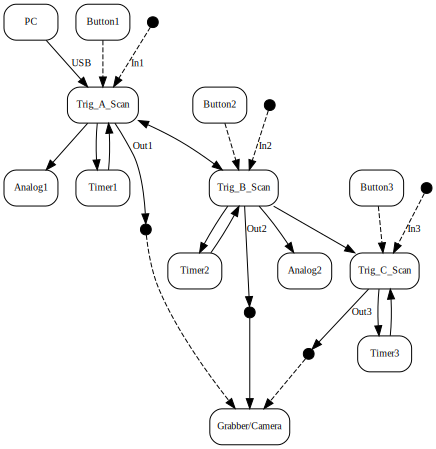
\includegraphics[height=105mm]{src/_Octane_Trigger_extended.pdf}
			% \caption{Trigger-structure.}
			% \label{_Octane_Trigger_extended}
		% \end{figure}

		\begin{figure}[ht]
			\centering
			\includegraphics[height=105mm]{src/_Octane_HW-Structure.pdf}
			\caption{Structure of the underlying hardware}
			\label{_Octane_HW-Structure.pdf}
		\end{figure}

% \spec{tag}{title}{module}{desc}
% \spec{}{}{}{}

	\spec{RI-}{Modules}{General}
	{ The Firmware has to be partitioned into these Modules:
		\begin{itemize}
		\item Main (Errorhandling)
		\item Triggers	(Timers)
		\item Sources	(SPI)
		\item Debug-Unit
		\item obs? System (WDG,CRC) 
		\item FSM (SCPI) 
		\item USB
		\item ResourceManager
		\item HAL (GPIO,WDG,CRC,DIO,UART,I2C,AIN)
		\item obs? Misc	(DIO,UART,I2C,AIN)
		\end{itemize}
	}

	\spec{RI-}{FSM-Module}{Main}
	{	the main-FSM has to implement the following functions
		\begin{itemize}
			\item 	uint8_t mainFSM() return 0 ... powerdown, -1 error, 1 ... reset, 2 ... restart
			\item 	bool parametrize(SCPI-ID, char * scpiString)
			\item 	bool processScpiID(SCPI-ID, char * scpiString)
		\end{itemize}
	}

	\spec{RI-}{FSM-States}{Main}
	{	the main-FSM has to implement the following states
		\begin{itemize}
		\item init
		\item running
		\item armed
		\item idling
		\item parametrizing 
		\item txUSB
		\item rxUsb
		\item errorState
		\end{itemize}
	}

	\spec{RI-}{ResMan}{General}
	{ All init()-Functions must probe the ResMan and only take and use a Resource when free. All deinit() - Functions must release Resources.}

	\spec{RI-}{Source-Modules}{Signals}
	{	16Bit-Voltage-Sources have to be accessible by following functions:
		\begin{itemize}
		\item 	\lstC !init() // not sure if necessary!
		\item 	\lstC !sendWord(bool source, uint16_t word)		// send 16Bit value over SPI to analog output!
		\item 	\lstC !loadArb(bool source, uint16_t size)!
		\item 	\lstC !scaleArb(bool source, uint16_t high, uint16_t low)! // rescale signal-vector vertically
		\item 	\lstC !loadRamp(bool source, uint16_t size, uint16_t high, uint16_t low)!
		\item 	\lstC !enab/disab analogue outputs A or B!
		\item 	\lstC !deinit() // not sure if necessary!
		\end{itemize}

		and following helper functions:
		\begin{itemize} \setlength\itemsep{1px}
			\item 	\lstC !float word2volt(uint16_t word) !
			\item 	\lstC !uint16_t	volt2word(float voltage) // -10V -> 0x00, 0 -> 30000, +10V -> 60000!
		\item 
		\end{itemize}

		and structures holding following data:
		\begin{itemize} \setlength\itemsep{1px}
		\item SPIx
		\item signalVector
		\item mode (triggered, detached, sinlgeshot)
		\item word min // upper vert. limit of ramp/arb
		\item word max // lower vert. limit of ramp/arb
		\item uint32	pulseTime
		\item 
		\end{itemize}
		
	}

	\spec{RI-}{scaling signals}{Signals}
	{	Vertically scaling of signal vectors will be applied irreversibly to signal-vectors in place.
		Amplitude, offset, high- and low-voltages are to be converted into min- and max-word and these again calculated onto existing vector values.
	}

	\spec{RI-}{writing signals}{Signals}
	{	Writing an arbitrary signal vector is only permitted in 'arbitrary'-mode. 
		Writing an arbitrary signal vector is complete if sufficient values were submitted and accepted.
		Writing an arbitrary signal vector can be aborted by setting the Sources mode to 'ramp'.
	}

	\spec{ RI- }{ResMan}{General}
	{ The FirmWare has to perform resource-management. This denotes to sanity-check managed resources being used by functionalities and deny functions if usage of resources would overlap.}

	\spec{ RI- }{ResourceList}{General}
	{ List of Resources to be managed:
		\begin{itemize} \setlength\itemsep{2px}
			\item Analogue Outputs, including SPIs, enable-Pins
			\item Analogue Inputs
			\item Digital Inputs/Outputs
			\item UART-Port
			\item I2C-Port
			\item Debug-Unit
			\item all processor-pins
		\end{itemize}
	}

	\spec{ RI- }{Debug-Unit}{Main}
	{ The Firmware has to implement a Debug-Unit, 8 digital outputs, that can be used to signalize certain events by setting/resetting/toggling them.
		Required functions are 
		\begin{itemize} \setlength\itemsep{1px}
		\item \lstC !initDbgUnit(void)  !
		\item \lstC !setDbgPinX(void)   !
		\item \lstC !clrDbgPinX(void)   !
		\item \lstC !tglDbgPinX(void)   !
		\item \lstC !deinitDbgUnit(void)!
		\end{itemize}
	}

	\spec{ RI- }{USB-Transceiver}{USB}
	{ The Firmware has to implement a USB-Transceiver for string-messages via VCP/CDC. Endpoints, to send and receive data have to established, as well as functions to access these endpoints.
		Required functions are 
		\begin{itemize} \setlength\itemsep{1px}
		\item \lstC !uint8_t CDC_Transmit_FS(uint8_t* Buf, uint16_t Len);!
		\item \lstC !// static int8_t CDC_Init_FS(void);!
		\item \lstC !// static int8_t CDC_DeInit_FS(void);!
		\item \lstC !// static int8_t CDC_Control_FS(uint8_t cmd, uint8_t* pbuf, uint16_t length);!
		\item \lstC !static int8_t CDC_Receive_FS(uint8_t* pbuf, uint32_t *Len);!
		\item \lstC !uint8_t newRxUSB(void);!
		\item \lstC !uint32_t lenRxUSB(void);!
		\item \lstC !void 	clrRxUSB(void);!
		\item \lstC !uint8_t *	getRxUSB(void);!
		\item \lstC !bool txUsb()!
		\item \lstC !initUsb()!
		\item \lstC !suspendUsb()!
		\item \lstC !resumeUsb()!
		\item \lstC !deinitUsb()!

		\end{itemize}
	}

	\spec{ RI- }{HAL-Module}{  }
	{ A hardware abstraction layer (HAL) has to be implemented, providing access to all necessary IO-Lines, serial-peripherals, the watchdog timer, cyclic-redundancy-check
	}

	\spec{ RI- }{HAL-Module}{  }
	{	must provide following interfacing functions:
		\begin{itemize} \setlength\itemsep{1px}
		\item initGPIOS()
		\item setPin()
		\item rstPin()
		\item getPin()
		\item deinitGPIOS()

		\item 
		\item initWDG(mode)
		\item setWDGtimeout()
		\item deinitWDG()

		\item initCRC()
		\item bool rxCRC(char * )
		\item txCRC(char * )
		\item deinitCRC()

		\item AIN, I2C, UART, DIO,
		\end{itemize}
		and following helper functions:
		\begin{itemize} \setlength\itemsep{1px}
		\item 
		\end{itemize}

		and structures holding following data:
		\begin{itemize} \setlength\itemsep{1px}
		\item 
		\end{itemize}

	}


	\spec{RI-}{scpi detection}{}
		{Implement USB-protocol in rSCPI.h, separately in short/longform, as well as an enum, representing the index of every command in the LUT.
		In the USB-ISR only mapping of the recieved string to a global variable and signaling to the FSM in main, that new data is to be processed happens, as well as sending out eventual Strings via USB.
		SCPI parsing in the FSM: looping over the SCPI-LUT and strncmp it to the input, until positive. Then either execute command immediately, or sscanf in the data. }

	\spec{}{scpi case-insensitive}{USB}
	{	\lstC !strncascmp()! ensures, that scpi-commands are detected case-insensitive
	}

	\spec{RI-}{thread-safe vriables}{main}{	Signalling between the FSM and the ISRs have to be thread-safe, and are therefore done via atomic operations, for example flags, semaphores or mutexes.
		Larger quantities of shared data, e.g. the signal vectors, are to be written, when the according ISR is deactivated, and may not be written on, while ISRs might read them. }

		\begin{figure}[ht]
			\centering
			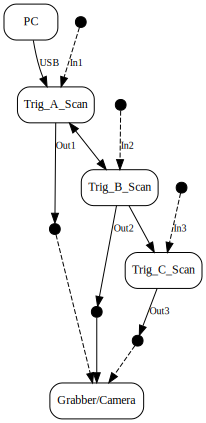
\includegraphics[height=105mm]{src/_Octane_Trigger_basic.pdf}
			\caption{Trigger-structure, basic concept.}
			\label{_Octane_Trigger_basic}
		\end{figure}
		\begin{figure}[ht]
			\centering
			\includegraphics[height=105mm]{src/_Octane_Trigger_extended_neato.pdf}
			\caption{Trigger-structure, extended concept.}
			\label{_Octane_Trigger_extended_kfdp}
		\end{figure}

	\spec{ RI- }{Naming Conventions}{ General }
	{	The following conventions shall be applied:
		\begin{itemize} \setlength\itemsep{1px}
		\item camelCase
		\item acting-Functions: 'verbNoun()'
		\item binary queries: 'is...()'
		\item 
		\end{itemize}
	}

	\spec{RI-}{naming convention}{General}
	{	naming scheme for digital IOs:
		\begin{itemize} \setlength\itemsep{1px}
			\item void	set<PinXY>();
			\item void	clr<PinXY>();
			\item bool	get<PinXY>();
		\end{itemize}
		e.g.:
		\begin{itemize} \setlength\itemsep{1px}
		\item void	setEN3();
		\item void	clrLED3();
		\item bool	getGPIO7();
		\end{itemize}
	}

	\spec{ RI- }{third party libs}{  }
	{	\begin{itemize} \setlength\itemsep{1px}
		\item CMSIS - ARM CoreM4 - Libraries
		\item stdbool.h
		\item usbdcdcif.h
		\item STM32F4 Pin- and Register-Defines
		\end{itemize}
	}


\begin{verbatim}
	
	K:\FH\MA\wim.txt durchforsten
	
	enums
		SourceA|B
		TrigA|B|C
	vars
	
	* Module:
		TestCases: mirror all the functionalities requested by User-requirements
		HAL Buttons, GPIOs, Relays, LEDs
		Miscellaneous - AnalogIN: Burst-mode wo ADCs die DAC-vektoren missbrauchen?
						- DIO
						- UART
						- I2C
		System	CRC, Wdg, Pwd/Rest/Rese/...

\end{verbatim}
	\spec{ RI- }{}{  }
	{	
	}

	\spec{ RI- }{opt pausing of Triggers}{  }
	{	Optional functionality: a falling Edge on a Trigger-In or pushing a dedicated Button (at red LED) during the running state, pauses or stops a whle Trigger-Sequence
	}

	\spec{ RI- }{rxUSB and parametrizing}{ USB-Stack }
	{	upon recieving a valid USB-packages, a parametrizazion-procedure has to be executed:
		validieren, applizieren, module updaten (Timers, Vektoren, Miscs ....)
		parametrize() - functions sits within the FSM Module and holds the long list of scpiID -> functions-calls
	}

	\spec{ RI- }{ISRs}{  }
	{	Necessary ISRs:
		\begin{itemize} \setlength\itemsep{1px}
		\item Buttons
		\item Timers for Triggers
		\item Trigger-Inputs
		\item UART, I2C, SPI
		\item USB
		\item Timer for Debounce
		\item Timer for Timeouts
		\end{itemize}
	}

	\spec{ RI- }{USB - safety}{  }
	{	USB-Inputs have to be sanity-checked regarding frequency, length and meaningful messages, as well as parameters within specified ranges

	}

	\spec{ RI- }{avoid reach-through}{ General }
	{	Timers, purposed for Triggers, are only to be accessed by their corresponding Trigger-unit.
		SPI-Ports are only to be accessed via their corresponding Source-Units.
	}

	\spec{ RI- }{ISR names}{ IRQs }
	{	Are defined in 'startup.....s'-assembler-file.	}

	\spec{ RI- }{Timer units}{ Timer }		% 2,8,3
	{	must provide following interfacing functions:
		\begin{itemize} \setlength\itemsep{1px}
			\item \lstC !bool initTimer(TIM_TypeDef * TIMx) // generic init to PWM-mode, no parameters!
			\item \lstC !bool setTimer(TIM_TypeDef * TIMx, uint32_t PSC, uint32_t ARR, uint32_t Pulse, uint32_t count)!
			\item \lstC !void startTimer(TIM_TypeDef * TIMx) enable IRQ!
			\item \lstC !void pauseTimer(TIM_TypeDef * TIMx) disableIRQ!
			\item \lstC !void stopTimer(TIM_TypeDef * TIMx) ?= reset(void) // pause(), reset counters, clearPin, zeroDAC()!
			\item \lstC !void deinitTimer(TIM_TypeDef * TIMx)	// generic deactivation of module!
			\item \lstC !void ISRs(void)!
		\end{itemize}
		and following helper functions:
		\begin{itemize} \setlength\itemsep{1px}
			\item timeStruct timerLUT(period)
			\item timeStruct timerHybrid(period) ... get PSC from LUT, calc ARR and pulse 
			\item $t_{samp}  = \frac{((PSC + 1)*(ARR+1))}{TCLK}$ -> $PSC = \frac{t_{samp} * TCLK }{(ARR+1)} - 1$
			% \item -> $t_{sampmin}  = \frac{((PSC + 1)( 0 + 1))}{TCLK} -> PSC + $
			% \item -> $t_{sampmax}  = \frac{((PSC + 1)( 2^{16} + 1))}{TCLK}$
			\item 	PSC-LUT: Zeitbereiche innerhalb derer ein PSC gilt, tmin $ = ((PSC + 1)*(0+1))/CLK$, tmax = $((PSC + 1)*(2^16+1))/CLK$ 
				\item 	jeder Eintrag in PSC-LUT ist eine union aus iTmin, iTmax, oPSC. timerHybrid() schleiferlt da drueber, bis passender \item 	PSC gefunden und rechnet daraus ARR und pulse
			\item timeStruct timerCALC(period) // timerFreq = Fclk/((PSC + 1)(ARR+1))
			\item $uint32\_t$ getTimerPSC(period) // LUT calculating PSC from given Timer-period: 0 for 4us ... 
		\end{itemize}

		and structures holding following data:
		\begin{itemize} \setlength\itemsep{1px}
		\item 	timeStruct: 	ARR, PSC, CCRx, ?length?
		\end{itemize}
	}

	\spec{ RI- }{Trigger units}{  }
	{	must provide following interfacing functions 
		\begin{itemize} \setlength\itemsep{1px}
		\item bool init(TRIG-ID, length, period, mode/input, , ...)
		\item arm(TRIG-ID)
		\item run(TRIG-ID) = start(TRIG-ID)
		\item pause(TRIG-ID)
		\item stop(TRIG-ID)
		\item reset(TRIG-ID)
		\item deinit(TRIG-ID)
		\end{itemize}

		and following helper functions:
		\begin{itemize} \setlength\itemsep{1px}
		\item nix, weil Timing in den Timer-Units berechnet wird
		\end{itemize}

		and structures holding following data:
		\begin{itemize} \setlength\itemsep{1px}
		\item TRIG-ID, TIM-ID
		\item state
		\item length, signal-period = time = 1/rate = 1/freq
		\item input/event-source
		\end{itemize}
	}

	\spec{ RI- }{ ResourceManager }{ Main }
	{	must provide following interfacing functions:
		\begin{itemize} \setlength\itemsep{1px}
		\item bool isTaken( <ResENUM> )
		\item bool take( <ResENUM> )
		\item void release( <ResENUM> )
		\end{itemize}
		and following helper functions:
		\begin{itemize} \setlength\itemsep{1px}
		\item 
		\end{itemize}

		and structures holding following data:
		\begin{itemize} \setlength\itemsep{1px}
		\item 	\lstC !ResENUM	{ RES_ 	RES_TRIGA 	RES_TRIGB 	RES_TRIGC 	RES_SOURCEA 	RES_SOURCEB 	RES_GPIO_E 	RES_UART 	
					  RES_I2C 	RES_SPI 	RES_ADC 	RES_Relay 	RES_TIMx 	RES_TIMx 	RES_TIMx 	RES_TIMx	RES_		}!
		\item 			Ausschlusstabelle zw Pins
		\end{itemize}
	}
			
	\spec{ RI- }{SPI units}{  }
	{	must provide following interfacing functions:
		\begin{itemize} \setlength\itemsep{1px}
		\item bool initSPI(SPIx) (in 16Bit Mode)
		\item txSpi(SPIx, word )
		\item word rxSpi(SPIx)
		\item deinitSPI(SPIx)
		\end{itemize}
		and following helper functions:
		\begin{itemize} \setlength\itemsep{1px}
		\item 
		\end{itemize}

		and structures holding following data:
		\begin{itemize} \setlength\itemsep{1px}
		\item 
		\end{itemize}

	}

	\spec{ RI- }{SCPI Module}{  }
	{	must provide following interfacing functions:
		\begin{itemize} \setlength\itemsep{1px}
		\item word getIDfromSCPIstring(char * scpiString, uint16 strLen)
		\end{itemize}

		and structures holding following data:
		\begin{itemize} \setlength\itemsep{1px}
		\item Stringlists containing recendt-shorts and -longs and norm-commands
		\item enum with exact same order as stringlists
		\item OR: \lstC !struct {longform, shortform, ID}! and for every ID a  \lstC !#define 0 TRIGA_STATE_OFF!
		\end{itemize}
	}

	% \spec{ RI- }{ units}{  }
	% {	must provide following interfacing functions:
		% \begin{itemize} \setlength\itemsep{1px}
		% \item init()
		% \item deinit()
		% \end{itemize}
		% and following helper functions:
		% \begin{itemize} \setlength\itemsep{1px}
		% \item 
		% \end{itemize}

		% and structures holding following data:
		% \begin{itemize} \setlength\itemsep{1px}
		% \item 
		% \end{itemize}

	% }

	\spec{ RI- }{Main module}{ Main }
	{	The firmware has to implement a main-Module, initializing all permanent modules (System-Clock, USB), activate the main-FSM and execute error-handling. It must provide following functions:
		\begin{itemize} \setlength\itemsep{1px}
		\item main(), including a super-loop and a call to the mainFSM
		\item ErrorHandler()
		\end{itemize}
		
		and structures holding following data:
		\begin{itemize} \setlength\itemsep{1px}
		\item scpi-identification string
		\item Processor Clock
		\item 
		\item 
		\end{itemize}

	}




	\spec{ RI- }{SysTick}{ main }
	{	A SysTick has to be established with a period of 10ms $\mu$s .
	}

	\spec{ RI- }{Clock}{ main }
	{	The Processor has to run at a frequency of 96MHz.
	}

	\spec{ RI- }{ms-Delay}{ main }
	{	The FW has to implement a loosely timed Delay function 
		\lstC !void delay_ms(int ms){     uint32 start=systickcount;    while (systickcount-start<ms); }!
	}

	\spec{ RI- }{Finite State Machine}{ main }
	{ The FW has to implement an event-driven FSM, that handles the necessary states, transitions and events according to figure \ref{fig:FSM} }

	\spec{ RI- }{LUT Signals}{ todo }
	{ The FW shall implement look-up-tables, 2 vectors, one for each Generator-channel, each at least of 2\textsuperscript{16} words(16bit) length, to contain user-defined waveforms for the Analog Outputs }

	\spec{ RI- }{Relais abstractions \label{relais}}{ todo }
	{ The FW shall implement functions to access relais, providing 'turn on', 'turn off' and 'retrieve status' }

	\spec{ RI- }{Abstraction of SignalGenerator-HW \label{absSigal}}{ todo }
	{ The FW shall implement functions to access the analog outputs, relying on the SPI-abstraction provided by REQ\ref{absFast} Enabling/disabling specified channels, setting specified voltage values.		}

	\spec{ RI- }{Abstraction of onboard-analogs \label{absADC}}{ todo }
	{ desc }

	\spec{ RI- }{Abstractions of highspeed digital IOs \label{absFast}}{ todo }
	{ The FW shall implement functions to manipulate and read the states of the Trigger IOs and SPI-channels and also to define them as outputs (initially), or inputs.}

	\spec{ RI- }{Abstractions of lowspeed digital IOs \label{absSlow}}{ todo }
	{ The FW shall implement functions to manipulate and read the states of the enable-lines of analog-outputs, and relay-lines and also to define them as outputs }

	\spec{ RI- }{Abstractions of misc. digital IOs }{ todo }
	{ The FW shall implement functions to manipulate and read the states of Buttons, Status-LEDs, Port3(8IOs), Port5(16IOs)  and also to define them as outputs (initially), or inputs. }

	\spec{ RI- }{ISR}{ General }
	{ The FW has to implement ISR-callbacks, to notice trigger-events on Button/Ext TriggerA...D, ISRs for TimersA,B and C, USBrx, ?USBtx? }

	\spec{ RI- }{Encoder/Stepper}{ todo }
	{ optional: The Firmware has to access available hardware to read encoder signals and send stepper commands. }

	\begin{table}[ht!]
	\centering
	\begin{tabular}{|l|c|l|l|l|l|}
	\hline
	\redrow Module	& Prio & Type	& Size 	& Purpose		& initial value \\ \hline
	% \hhline{======}                         	
	FSM			& H	& struct	& 			& 					& 		\\ \hline
			% 	& M	& enum		& -			& statePrev			& INIT	\\ \hline
				& H	& enum		& -			& state				& INIT	\\ \hline
				& M	& enum		& -			& stateNext			& INIT	\\ \hline
				& H	& flag		& -			& inUSBnew			& low	\\ \hline
				& H	& flag		& -			& outUSBnew			& low	\\ \hline
	USB-Stack	& H	& struct	& 			& 					& 		\\ \hline
				& H	& string	& 			& inUSB				& empty	\\ \hline
				& H	& string	& 			& outUSB			& empty	\\ \hline
				& H	& 			& 			& max. String lenght		& 		\\ \hline
	SCPI		& H	& 			& 			& 					& 		\\ \hline
				& H	& str-list	& 			& SCPI commands	lon & 		\\ \hline
			%	& H	& str-list	& 			& SCPI commands	sho & 		\\ \hline
				& H	& str-list	& 			& SCPI responses	& 		\\ \hline
				& H	& str-list	& 			& error codes		& 		\\ \hline
				& H	& enum		& 			& command coding	& 		\\ \hline
	Trigger A	& H	& struct	& 			& 					& 		\\ \hline
	Trigger B	& H	& struct	& 			& 					& 		\\ \hline
	Trigger C	& H	& struct	& 			& 					& 		\\ \hline
	Generator 1	& H	& struct	& 			& 					& 		\\ \hline
				& H	& 16 bit	& $>2^{16}$	& Signal-Vector		& 0s	\\ \hline
	Generator 2	& H	& struct	& 			&					& 		\\ \hline
				& H	& 16 bit	& $>2^{16}$	& Signal-Vector		& zeroes\\ \hline
	Relais 1..8	& H	& structs	& 			& 					& 		\\ \hline
	Watchdog	& H	& struct	& 			& 					& 		\\ \hline
	CRC			& H	& struct	& 			& 					& 		\\ \hline
	IO-Lines	& H	& structs	& 			& 					& 		\\ \hline
	% Peripherals	& H	& structs	& 			& 					& 		\\ \hline
			\end{tabular}
		\caption{Required data inside the FW.}
	\label{tab:Vars}
	\end{table}
	
	\spec{RI-}{how to Trigger}{Triggers}
	{	\begin{itemize}
		\item A Trigger Event is either a SCPI-Command "TRIGx:STAT:RUN", an external logic Signal on signal-line TRIGx, or by pressing the button BUTTx, or, in linked mode, issued by the superior Trigger. 
		\item A Trigger Event causes the according Timer-Interrupt to be enabled. The affected Trigger-unit then, runs for a number of steps specified by "TRIGx:COU count", with a speed defined by "TRIG0:TIME time" or "TRIGx:FREQ freq", and after that disables its own Interrupt. 
		\item Activation of at least one Trigger causes the USB-Interrupt to be deactivated, to ensure no interference with the critical timing of Triggering and Signal Generation. Unless Trigger a or B have a duration of at least 2 seconds, or at least one Trigger has a Step-Count of '0',in which case USB-Interrupt needs to be active, otherwise, the whole OCTane would be frozen for too long. 
		\item Every step, the Trigger pulses its own Trigger-Output line, reads the recent value from its Generators LUT and sends that value to the Gen via SPI, increases the step count and potentially triggers its inferior Trigger. 
		\item In linked mode, the superior unit enables the IRQ of the inferior. In independent mode, a button, an ext Trigger, or the SCPI-Command triggers an IRQ. 
		\end{itemize}
	}

		\begin{table}[H]
			\centering
			\begin{tabular}{|l|l|l|l|l|l|}
			\hline
			\redrow Function		& Prio 	& Port	& HW-Identifier 			& Type	& initial value \\ \hline
					Trigger 1		& high 	& A		& $TRIG\_1$	& digital IO, HighSpeed		& low		\\ \hline
					Trigger 2		& high 	& B		& $TRIG\_2$	& digital IO, HighSpeed		& low		\\ \hline
					Trigger 3		& high 	& B		& $TRIG\_3$	& digital IO, HighSpeed		& low		\\ \hline
					Trigger 4		& high 	& B		& $TRIG\_4$	& digital IO, HighSpeed		& low		\\ \hline
					SPI 1			& high 	& A		& $SCLK\_1, NSS\_1, MISO\_1, MOSI\_1$	& Serial Peripheral IF, HighSpeed		& 0x0000		\\ \hline
					SPI 2			& high 	& B		& $SCLK\_2, NSS\_2, MISO\_2, MOSI\_2$	& Serial Peripheral IF, HighSpeed		& 0x0000		\\ \hline
					Relais, SLD		& high 	& D		& $GPIO\_8$	& digital out, LowSpeed		& low		\\ \hline
					Relais, AIM		& high 	& D		& $GPIO\_7$	& digital out, LowSpeed		& low		\\ \hline
					Relais, CAM		& high 	& D		& $GPIO\_6$	& digital out, LowSpeed		& low		\\ \hline
					Relais, Galvo	& high 	& D		& $GPIO\_5$	& digital out, LowSpeed		& low		\\ \hline
					State LED, 1	& low 	& D		& $STATE\_1$	& digital out, LowSpeed	& low		\\ \hline
					State LED, 2	& low 	& D		& $STATE\_2$	& digital out, LowSpeed	& low		\\ \hline
					State LED, 3	& low 	& D		& $STATE\_3$	& digital out, LowSpeed	& low		\\ \hline
					State LED, 4	& low 	& D		& $STATE\_4$	& digital out, LowSpeed	& low		\\ \hline
					PushButton, 1	& mid 	& D		& $BUTT\_1$	& digital in, LowSpeed			& n.a.		\\ \hline
					PushButton, 2	& mid 	& D		& $BUTT\_2$	& digital in, LowSpeed			& n.a.		\\ \hline
					PushButton, 3	& mid 	& D		& $BUTT\_3$	& digital in, LowSpeed			& n.a.		\\ \hline
					PushButton, 4	& mid 	& D		& $BUTT\_4$	& digital in, LowSpeed			& n.a.		\\ \hline
					enable Analog1	& high 	& C		& $EN\_1$	& digital out, LowSpeed		& low		\\ \hline
					enable Analog2	& high 	& C		& $EN\_2$	& digital out, LowSpeed		& low		\\ \hline
					Analog in 1		& low 	& C		& $ADC\_1$	& analog In		& n.a.		\\ \hline
					Analog in 2		& low 	& C		& $ADC\_2$	& analog In		& n.a.		\\ \hline
					Analog in 3		& low 	& C		& $ADC\_3$	& analog In		& n.a.		\\ \hline
					Analog in 4		& low 	& C		& $ADC\_4$	& analog In		& n.a.		\\ \hline
					USB				& high 	& -		& $USB\_FS\_DM$	& USB Data-		& n.a.		\\ \hline
					USB				& high 	& -		& $USB\_FS\_DP$	& USB Data+		& n.a.		\\ \hline
					USB				& high 	& -		& $USB\_FS\_ID$	& USB ident.	& n.a.		\\ \hline
					\end{tabular}
					\caption{Mapping of IO-lines.}
					\label{tab:Mapping}
		\end{table}



	\section{Implementation}	
\subsection{Modules}	
	
	\begin{itemize} \setlength\itemsep{1px}
		\item Main.h/.c (Errorhandling)
		\item ResourceMan.h/.c
		\item Triggers.h/.c
		\item Timers.h/.c
		\item Sources.h/.c
		\item DebugUnit.h/.c
		\item FSM.h/.c
		\item SCPI.h/.c
		\item USB
		\item HAL (GPIO, SPI)
		\item Misc.h/.c	(WDG,CRC,DIO,UART,IRC,AIN)
		\item or: HAL (GPIO, SPI, WDG,CRC,DIO,UART,IRC,AIN)
	\end{itemize}




	\pagebreak
	\section{USB-Protocol for OCTane (SCPI)}
				\begin{longtable}{|l|l|l|l|l|}				\hline
		Sub-sys				& Parameter		& Value					& Command									& Response 			\\ \hline
		\redrow	Trigger A	& State			& off|idle|arm|run		& TRIGgerA:STATe	OFF						& <state>|<error>	\\ \hline
							& State			& 						& TRIGgerA:STATe	IDLE					& <state>|<error>	\\ \hline
							& State			& 						& TRIGgerA:STATe	ARM						& <state>|<error>	\\ \hline
							& State			& 						& TRIGgerA:STATe	RUN						& <state>|<error>	\\ \hline
							& Mode (freerun)& finite				& TRIGgerA:MODE		FINite					& <mode> |<error>	\\ \hline
							& Mode 			& infinite				& TRIGgerA:MODE		INFinite				& <mode> |<error>	\\ \hline
							& Input			& USB					& TRIGgerA:INput	USB						& <input>|<error>	\\ \hline
							& Input			& external input		& TRIGgerA:INput	EXTernal				& <input>|<error>	\\ \hline
							& Input			& Trigger B				& TRIGgerA:INput	TRIGgerB				& <input>|<error>	\\ \hline
							& Input			& Trigger C				& TRIGgerA:INput	TRIGgerC				& <input>|<error>	\\ \hline
							& Input			& Button				& TRIGgerA:INput	BUTTon					& <input>|<error>	\\ \hline
							& Signal-Rate	& 1.0e-1 ... 125e3		& TRIGgerA:RATE		<freq>					& <time>|<error>	\\ \hline
							& Signal-Period	& 	8e-6	... 10		& TRIGgerA:PERIod	<time>					& <time>|<error>	\\ \hline
							& Vector-Size	& 1...250000			& TRIGgerA:SIZE		<size>					& <size>|<error>	\\ \hline
		%	Sequencer		& -Gener		& 						& TRIGgerA:									& DONE|		\\ \hline
		\redrow	Trigger B	& State			& off|idle|arm|run		& TRIGgerB:STATe	OFF						& <state>|<error>	\\ \hline
							& State			& 						& TRIGgerB:STATe	IDLE					& <state>|<error>	\\ \hline
							& State			& 						& TRIGgerB:STATe	ARM						& <state>|<error>	\\ \hline
							& State			& 						& TRIGgerB:STATe	RUN						& <state>|<error>	\\ \hline
							& Mode (freerun)& finite				& TRIGgerB:MODE		FINite					& <mode> |<error>	\\ \hline
							& Mode 			& infinite				& TRIGgerB:MODE		INFinite				& <mode> |<error>	\\ \hline
							& Input			& USB					& TRIGgerB:INput	USB						& <input>|<error>	\\ \hline
							& Input			& External				& TRIGgerB:INput	EXTernal				& <input>|<error>	\\ \hline
							& Input			& Trigger C				& TRIGgerB:INput	TRIGgerC				& <input>|<error>	\\ \hline
							& Input			& Button				& TRIGgerB:INput	BUTTon					& <input>|<error>	\\ \hline
							& Signal-Rate	& 	1.0e-1 ... 125e3	& TRIGgerB:RATE		<freq>					& <time>|<error>	\\ \hline
							& Signal-Period	& 	8e-6	... 10		& TRIGgerB:PERIod	<time>					& <time>|<error>	\\ \hline
							& Vector-Size	& 1...250000			& TRIGgerB:SIZE		<size>					& <size>|<error>	\\ \hline
		%	Sequencer		& -Gener		& 						& TRIGgerB:									& DONE|		\\ \hline
		\redrow	Trigger C	& State			& off|idle|arm|run		& TRIGgerC:STATe	OFF						& <state>|<error>	\\ \hline
							& State			& 						& TRIGgerC:STATe	IDLE					& <state>|<error>	\\ \hline
							& State			& 						& TRIGgerC:STATe	ARM						& <state>|<error>	\\ \hline
							& State			& 						& TRIGgerC:STATe	RUN						& <state>|<error>	\\ \hline
							& Mode (freerun)& finite				& TRIGgerC:MODE		FINite					& <mode> |<error>	\\ \hline
							& Mode 			& infinite				& TRIGgerC:MODE		INFinite				& <mode> |<error>	\\ \hline
							& Input			& USB					& TRIGgerC:INput	USB						& <input>|<error>	\\ \hline
							& Input			& External				& TRIGgerC:INput	EXTernal				& <input>|<error>	\\ \hline
							& Input			& Button				& TRIGgerC:INput	BUTTon					& <input>|<error>	\\ \hline
							& Signal-Rate	& 	1.0e-1 ... 125e3	& TRIGgerC:RATE		<freq>					& <time>|<error>	\\ \hline
							& Signal-Period	& 	8e-6	... 10		& TRIGgerC:PERIod	<time>					& <time>|<error>	\\ \hline
							& Vector-Size	& 1...250000			& TRIGgerC:SIZE		<size>					& <size>|<error>	\\ \hline
						% 	& Slope			& rising|falling Edge	& TRIGgerC:SLOPe	<POS|NEG>				& DONE|		\\ \hline
						% 	& Outmode		& pulse|duty			& TRIGgerC:OUTMode	<pulse|duty>			& DONE|		\\ \hline
						% 	& Outpulse		& pulse|duty			& TRIGgerC:OUTPulse	<time>					& DONE|		\\ \hline
						% 	& OutSlope		& rising|falling Edge	& TRIGgerC:OUTSLope	<POS|NEG>				& DONE|		\\ \hline
		%	Sequencer		& -Gener		& 						& TRIGgerC:									& DONE|		\\ \hline
		\redrow	Source-A	& Mode			& triggered				& SOURceA:MODE			TRIGgered			& <mode>|<error> 	\\ \hline
							& Mode			& detached				& SOURceA:MODE			DETached			& <mode>|<error> 	\\ \hline
							& Mode			& singleshot			& SOURceA:MODE			SINGleshot			& <mode>|<error> 	\\ \hline
							& Function		& Ramp					& SOURceA:FUNCtion:SHAPe 	RAMP	 		& <func>|<error>	\\ \hline
							& Function		& 		Arbitrary		& SOURceA:FUNCtion:SHAPe 	ARBitrary 		& <func>|<error>	\\ \hline
							& Symmetry		& 0 ... 100 			& SOURceA:RAMP:RATIO 	<ratio> 			& <ratio>|<error> 	\\ \hline
							& Arb load		& -						& SOURceA:ARBitrary:LOAD 					& <count>|<error>	\\ \hline
							& Arb val		& $\pm$10.000			& SOURceA:ARBitrary:VALUe <idx, val>		& <idx, val>|<error>\\ \hline
							& Amplitude		& 0.000...20.000		& SOURceA:FUNCtion:AMPlitude <ampl>			& <ampl>|<error>	\\ \hline
							& Offset		& $\pm$10.000			& SOURceA:FUNCtion:OFFset <offs>			& <offs>|<error>	\\ \hline
							& High			& $\pm$10.000			& SOURceA:FUNCtion:HIgh <high>				& <high>|<error>	\\ \hline
							& Low			& $\pm$10.000			& SOURceA:FUNCtion:LOw <low>				& <low>|<error> 	\\ \hline
							& Constant		& $\pm$10.000			& SOURceA:VOLTage:LEVel	<volts>				& <volts>|<error> 	\\ \hline
							& Timeout		&  1...1000ms		 	& SOURceA:PULSe:WIDth		<time>			& <time>|<error> 	\\ \hline
						% 	& ReadVec		& -						& SOURceA:ARBitrary:READ					& all vector values \\ \hline
		\redrow	Source-B	& Mode			& trig|det|single		& SOURceB:MODE			TRIGgered			& <mode>|<error> 	\\ \hline
							& Mode			& trig|det|single		& SOURceB:MODE			DETached			& <mode>|<error> 	\\ \hline
							& Mode			& trig|det|single		& SOURceB:MODE			SINGleshot			& <mode>|<error> 	\\ \hline
							& Function		& Ramp					& SOURceB:FUNCtion:SHAPe 	RAMP	 		& <func>|<error>	\\ \hline
							& Function		& Arbitrary				& SOURceB:FUNCtion:SHAPe 	ARBitrary 		& <func>|<error>	\\ \hline
							& Symmetry		& 0 ... 100 			& SOURceB:RAMP:RATIO 	<ratio> 			& <ratio>|<error> 	\\ \hline
							& Arb load		& -						& SOURceB:ARBitrary:LOAD 					& <count>|<error>	\\ \hline
							& Arb val		& $\pm$10.000			& SOURceB:ARBitrary:VALUe <idx, val> 		& <idx, val>|<error>\\ \hline
							& Amplitude		& 0.000...20.000		& SOURceB:FUNCtion:AMPlitude <ampl>			& <ampl>|<error>	\\ \hline
							& Offset		& $\pm$10.000			& SOURceB:FUNCtion:OFFset <offs>			& <offs>|<error>	\\ \hline
							& High			& $\pm$10.000			& SOURceB:FUNCtion:HIgh <high>				& <high>|<error>	\\ \hline
							& Low			& $\pm$10.000			& SOURceB:FUNCtion:LOw <low>				& <low>|<error> 	\\ \hline
							& Constant		& $\pm$10.000			& SOURceB:VOLTage:LEVel	<volts>				& <volts>|<error> 	\\ \hline
							& Timeout		&  1...1000ms		 	& SOURceB:PULSe:WIDth		<time>			& <time>|<error> 	\\ \hline
						% 	& ReadVec		& -						& SOURceB:ARBitrary:READ					& all vector values \\ \hline
		% \redrow	Misc.		& 				& 						& 											&  					\\ \hline
			Relays			& Galvo			& close|open|read		& ROUTe:<CLOSe|OPEN|STATE?> GAL				& <state>|<error>	\\ \hline
							& SLD			& close|open|read		& ROUTe:<CLOSe|OPEN|STATE?> SLD				& <state>|<error>	\\ \hline
							& AIM			& close|open|read		& ROUTe:<CLOSe|OPEN|STATE?> AIM				& <state>|<error>	\\ \hline
							& CAM			& close|open|read		& ROUTe:<CLOSe|OPEN|STATE?> CAM				& <state>|<error>	\\ \hline
						% 	& Sense			& read state			& ROUTe:STATE?	GAL|SLD|AIM|CAM				& <state>|<error>	\\ \hline
						% 	& close			& close Relay			& ROUTe:CLOSe	GAL|SLD|AIM|CAM				& <state>|<error>	\\ \hline
						% 	& open			& open Relay			& ROUTe:OPEN	GAL|SLD|AIM|CAM				& <state>|<error>	\\ \hline
			I2C				& mode			& OFF					& I2C::MODE OFF								& <mode>|<error>	\\ \hline
							& mode			& USB					& I2C::MODE USB								& <mode>|<error>	\\ \hline
							& mode			& slave-action			& I2C::MODE SLAVeaction						& <mode>|<error>	\\ \hline
							& write			& 0 ... 255				& I2C::WRITe <val>							& <val>|<error> 	\\ \hline
							& read			& 0 ... 255				& I2C::READ									& <val>|<error> 	\\ \hline
			UART			& mode			& OFF					& UART:MODE OFF								& <mode>|<error> 	\\ \hline
							& mode			& USB					& UART:MODE USB								& <mode>|<error> 	\\ \hline
							& mode			& slave-IRQ				& UART:MODE SLAVeaction						& <mode>|<error> 	\\ \hline
							& write			& 0 ... 255				& UART:WRITe <val>							& <val>|<error>		\\ \hline
							& read			& 0 ... 255				& UART:READ									& <val>|<error> 	\\ \hline
			DIO				& mode			& OFF			 		& DIGIO:MODE OFF							& <val>|<error>		\\ \hline
							& mode			& input			 		& DIGIO:MODE IN								& <val>|<error>		\\ \hline
							& mode			& output 				& DIGIO:MODE OUT							& <val>|<error>		\\ \hline
							& write			& 0 .. 65535			& DIGIO:WRIte <val>							& <val>|<error>		\\ \hline
							& read			& 0 .. 65535			& DIGIO:READ								& <val>|<error>		\\ \hline
			AnalogIN		& mode			& OFF					& ANAlog0|1|2|3:MODE OFF					& <val>|<error>		\\ \hline
							& mode			& USB					& ANAlog0|1|2|3:MODE USB					& <val>|<error>		\\ \hline
							& mode			& triggered				& ANAlog0|1|2|3:MODE TRIGA					& <val>|<error>		\\ \hline
							& mode			& triggered				& ANAlog0|1|2|3:MODE TRIGB					& <val>|<error>		\\ \hline
							& mode			& triggered				& ANAlog0|1|2|3:MODE TRIGC					& <val>|<error>		\\ \hline
							& read			& 0 ... 4095			& ANAlog0|1|2|3:READ						& <val>|<error>		\\ \hline
		\redrow System		& CRCmode		& OFF					& SYStem:CRC16 OFF							& <state>|<error>	\\ \hline
							& CRCmode		& on					& SYStem:CRC16 ON							& <state>|<error>	\\ \hline
							& ShutDown 		& -						& SYStem:POWerdown							& POWD|<error>	\\ \hline
							& ListSCPI 		& -						& SYStem:LISt								& <list>|<error>	\\ \hline
							& RESEt 		& -						& SYStem:RESEt								& RESE|<error>		\\ \hline
							& RESTart 		& -						& SYStem:RESTart							& REST|<error>	\\ \hline
							& Verbosity		& OFF					& SYStem:VERBose OFF						& <mode>|<error>	\\ \hline
							& Verbosity		& on					& SYStem:VERBose ON							& <mode>|<error>	\\ \hline
							& Watchdog		& OFF					& SYStem:WATchdog OFF						& <mode>|<error>	\\ \hline
							& Watchdog		& on					& SYStem:WATchdog ON						& <mode>|<error>	\\ \hline
							& Time			& 1...1000ms			& SYStem:WATchdog <time>					& <time>|<error>	\\ \hline
			% Encoder		& 	opt. 		& 						& 												& 		& 		\\ \hline
			% Stepper		& 	opt. 		& 						& 												& 		& 		\\ \hline
		\caption{OCTane USB-protocol, commands.}
			\end{longtable}

		% \begin{table}[h!]
			\centering
			\begin{longtable}{|l|l|l|l|l|l|}
			% \begin{tabular}{|p{1.6cm}|l|l|l|l|l|}
			\hline


		Sub-sys					&  Parameter	 	& possible messages	& occurence 						& 			&  \\ \hline
		\redrow	Trigger A|B|C	&  State	 		& TrigX idling|armed|running& sent on every state change 		& 			& 	\\ \hline
				Trigger A|B|C 	& Input				& -200				& error, if button in use			& 			& 	\\ \hline
				Trigger A|B|C 	& Signal-Rate		& -200				& error, if out-of-range			& 			& 	\\ \hline
				Trigger A|B|C 	& Signal-Period		& -200				& error, if out-of-range			& 			& 	\\ \hline
				Trigger A|B|C 	& Vector-Size		& -200				& error, if out-of-range			& 			& 	\\ \hline
		\redrow	Source A|B		& Arb load	 		& -200				& error, if not in Arb-mode			& 			& 	\\ \hline
				Source A|B		& Arb val	 		& VectorX complete	& if sufficient amount of values was sent	& 			& 	\\ \hline
				Source A|B		& Arb val	 		& -200				& error, if out-of-range			& 			& 	\\ \hline
				Source A|B		& Arb val	 		& -200				& error, if exeeds vector-size		& 			& 	\\ \hline
				Source A|B		& Symmetry	 		& -200				& error, if out-of-range			& 			& 	\\ \hline
				Source A|B		& Amplitude			& -200				& error, if out-of-range			& 			& 	\\ \hline
				Source A|B		& Offset			& -200				& error, if out-of-range			& 			& 	\\ \hline
				Source A|B		& High				& -200				& error, if out-of-range			& 			& 	\\ \hline
				Source A|B		& Low				& -200				& error, if out-of-range			& 			& 	\\ \hline
				Source A|B		& Constant			& -200				& error, if out-of-range			& 			& 	\\ \hline
				Source A|B		& Timeout			& -200				& error, if out-of-range			& 			& 	\\ \hline

		\redrow	AIN 			& input value		& AINx: <value>		& sent on every corresp. Trigger	& 			& 	\\ \hline
				DIN 			& input value		& DIN: <value>		& sent on every DIO:READ-Command	& 			& 	\\ \hline
				UART 			& input value		& UART: <value>		& sent on every corresp. Trigger	& 			& 	\\ \hline
				I2C 			& input value		& I2C: <value>		& sent on every corresp. Trigger	& 			& 	\\ \hline
		\caption{OCTane USB-protocol, responses.}
		\label{USB-Protocol-responses}
		\end{longtable}
		% \end{table}

				\begin{longtable}{|l|l|l|l|l|}				\hline
			Command & 	Description									& 	Action	& Return		\\ \hline
			*CLS	& Clear Status Command							& 		& 		\\ \hline
			*ESE & Standard Event Status Enable Command	& 		& 		\\ \hline
			*ESE? & Standard Event Status Enable Query 		& -		& 		\\ \hline
			*ESR? & Standard Event Status Register Query 	& -		& 		\\ \hline
			*IDN? & Identification Query 							& 	-	& ID-String \\ \hline
			*OPC & Operation Complete Command 				& 		& 		\\ \hline
			*OPC? & Operation Complete Query 					& 	-	& 		\\ \hline
			*RST & Reset Command 									& 		& 		\\ \hline
			*SRE & Service Request Enable Command 			& 		& 		\\ \hline
			*SRE? & Service Request Enable Query 				& 	-	& 		\\ \hline
			*STB? & Read Status Byte Query 						& 	-	& Status Byte		\\ \hline
			*TST? & Self-Test Query 									& 	-	& 		\\ \hline
			*WAI & Wait-to-Continue Command 					& 		& 		\\ \hline
			\caption{IEEE 488.2 mandatory commands}
		\end{longtable}
		
		% \begin{longtable}{|l|l|l|l|l|}				\hline
			% Command & 	Description									& 	Action	& Return		\\ \hline
			% *AAD & Accept Address Command						& 		& 		\\ \hline
			% *CAL? & Calibration Query								& 		& 		\\ \hline
			% *DDT & Define Device Trigger Command				& 		& 		\\ \hline
			% *DDT? & Define Device Trigger Query					& 		& 		\\ \hline
			% *DLF & Disable Listener Function Command		& 		& 		\\ \hline
			% *DMC & Define Macro Command						& not imp'd & 		\\ \hline
			% *EMC & Enable Macro Command						& not imp'd & 		\\ \hline
			% *EMC? & Enable Macro Query							& not imp'd & 		\\ \hline
			% *GMC? & Get Macro Contents Query 					& 		& 		\\ \hline
			% *IST? & Individual Status Query						& 		& 		\\ \hline
			% *LMC? & Learn Macro Query								& not imp'd & 		\\ \hline
			% *LRN? & Learn Device Setup Query					& 		& 		\\ \hline
			% *OPT? & Option Identification Query					& 		& 		\\ \hline
			% *PCB & Pass Control Back									& 		& 		\\ \hline
			% *PMC & Purge Macros Command						& not imp'd & 		\\ \hline
			% *PRE & Parallel Poll Enable Register Command	& 		& 		\\ \hline
			% *PRE? & Parallel Poll Enable Register Query		& 		& 		\\ \hline
			% *PSC & Power-On Status Clear Command			& 		& 		\\ \hline
			% *PSC? & Power-On Status Clear Query				& 		& 		\\ \hline
			% *PUD & Protected User Data Command				& 		& 		\\ \hline
			% *PUD? & Protected User Data Query					& 		& 		\\ \hline
			% *RCL & Recall Command									& 		& 		\\ \hline
			% *RDT & Resource Description Transfer Command	& 		& 		\\ \hline
			% *RDT? & Resource Description Transfer Query		& 		& 		\\ \hline
			% *SAV & Save Command									& 		& 		\\ \hline
			% *TRG & Trigger Command									& 		& 		\\ \hline
			% *RMC & Remove Individual Macro Command		& not imp'd & 		\\ \hline
			% *SDS & Save Default Device Settings Command	& 		& 		\\ \hline
			% \caption{IEEE 488.2 optional commands}
		% \end{longtable}

	\pagebreak
	\section{Standard operating procedures}
		\TODO{update to new protocol}
			{	\begin{table}[h!]
		\scriptsize
			 \begin{tabular}{|p{5.5cm}|p{6cm}|} \hline
			SOURce1:FUNCtion:Amplitude 6	&	\\ \hline
			SOURce1:FUNCtion:Offset 3		&	\\ \hline
			SOURce2:FUNCtion:Amplitude 4	&	\\ \hline
			SOURce2:FUNCtion:Offset -4		&	\\ \hline
			TRIGgerC:STATe RUN				&	start scan sequence\\ \hline
			 \end{tabular}
			 \caption{One volume-scan.}
		\end{table}
	}
		\begin{table}[h!]
		\scriptsize
			 \begin{tabular}{|p{5.5cm}|p{6cm}|} \hline
			SOUR2:VOLT:LEV 4.5		& both Galvos in fixed positions	\\ \hline
			SOUR1:VOLT:LEV -2.95	& no Triggers	\\ \hline
			...	& 	\\ \hline
			SOUR2:VOLT:LEV 0	& Send galvos home afterwards	\\ \hline
			SOUR1:VOLT:LEV 0	& 	\\ \hline
			 \end{tabular}
			 \caption{A-scan in one position.}
		\end{table}

		\begin{table}[h!]
		\scriptsize
			 \begin{tabular}{|p{5.5cm}|p{6cm}|} \hline
			 % \end{tabular}
			 % \caption{ }
		% \end{table}
		% \begin{table}[h!]
			 % \begin{tabular}{|p{5.5cm}|p{6cm}|} \hline
			TRIGgerB:STATe stop	& deactivate	\\ \hline
			TRIGgerA:STATe stop	& in exactly this order	\\ \hline
			SOUR1:VOLT:LEV 0	& send Galvo home	\\ \hline
			SOUR1:mode:trig		& reattach Galvo to TriggerB	\\ \hline
			TRIGgerB:MODE trigC & reattach TriggerB to TriggerC \\ \hline
			 \end{tabular}
			 \caption{B-scan in one position, continuous A-scans, 'freerun-mode'.}
		\end{table}
		% \begin{table}[h!]
		% \scriptsize
			 % \begin{tabular}{|p{5.5cm}|p{6cm}|} \hline
			% SOUR1:MODE free				& detach Galvo from its Trigger	\\ \hline
			% SOURce2:FUNCtion:Amplitude 3.5	& 	\\ \hline
			% SOURce2:FUNCtion:Offset 1.95	& 	\\ \hline
			% TRIGgerB:Mode CONTinuous	& ...Trigger will run forever	\\ \hline
			% TRIGA:PRE 4	& 	\\ \hline
			% TRIGA:tcou 74	&	...40kHz A-Scans	\\ \hline
			% TRIGB:pre 64	&		....10Hz B-Scans 	\\ \hline
			% TRIGA:cou 1550 	& 1550 samples	\\ \hline
			% TRIGB:tcou 36500 	& 10Hz 	\\ \hline
			% TRIGgerB:STATe RUN	& activate	\\ \hline
								% & 			\\ \hline
			% TRIGgerB:STATe stop	& activate	\\ \hline
			% TRIGA:cou 1250 	& 1250 samples	\\ \hline
			% TRIGB:tcou 14600	& 25Hz 	\\ \hline
			% TRIGgerB:STATe RUN	& activate	\\ \hline
								% & 			\\ \hline
			% TRIGgerB:STATe stop	& deactivate	\\ \hline
			% TRIGA:cou 620 	& 620 samples	\\ \hline
			% TRIGB:tcou 7300	& 50Hz 	\\ \hline
			% TRIGgerB:STATe run	& activate	\\ \hline
								% & 			\\ \hline
			% TRIGgerB:STATe stop	& deactivate in exactly	\\ \hline
			% TRIGgerA:STATe stop	& this order	\\ \hline
			% SOUR1:VOLT:LEV 0	& send Galvo home	\\ \hline
			% SOUR1:mode:trig		& reattach Galvo to TriggerB	\\ \hline
			% TRIGgerB:MODE trigC & reattach TriggerB to TriggerC \\ \hline
			 % \end{tabular}
			 % \caption{Ivan Patch }
		% \end{table}	


	\section{Constraints, Assumptions}

	
			Usage of the Processor STM32F407VGT6 imposes following relevant constraints:
			\begin{itemize}
				\item max. clock speed 72MHz
				\item 1MB program memory
				\item max. 82 IO-channels
			\end{itemize}
			

			% Utilization of these ressources:
			% \begin{itemize}
			% \item A maximum clock speed of 72MHz and SPI-channels, for the analog outputs, with a datarate of up to 2 Mbyte/s, ensure the required max. frequency for A-scans of 250kHZ to be feasible.
			
			% \item An estimate of 300kByte of memory necessary for the FWs algorithms and data, including timetable and SCPI-LUT, as well as 2 vectors within the FW, to hold the analog waveforms of 2x 256kbyte, leave a remainder of \~ 200kByte within the Processors program memory.

			% \item Usage of the available IO-lines follows the following table, ensuring all relevant communication with other components of the OCT-system is represented. 
			% \end{itemize}
			
	% \subsection{Dependencies, Guidelines}

	
	\subsection{Reference Documents}
	\subsection{Abbreviations and Acronyms}
			\section{Abbreviations and Acronyms}
	\begin{table}[h!]
			\begin{tabular}{|p{2cm}|l|}
			\hline	
			uC		& MicroController							\\ \hline
			FW		& Firmware, the Software, running on the uC \\ \hline	
			OCT		& Optical Coherence Tomography				\\ \hline	
			SW		& Software, the Software, running on the OCT-System 	\\ \hline	
			FSM 	& Finite State Machine									\\ \hline
			CRC		& Cyclic Redundancy Check								\\ \hline
			IO		& Input-Output, bidirectional Communcation Lines 		\\ \hline
			USB		& Universal Serial Bus									\\ \hline
			VCP		& Virtual Com Port, a serial connection via USB			\\ \hline
			% CDC		& communications device class, implements VCP over USB	\\ \hline
			USB		& Universal Serial Bus									\\ \hline
			SCPI	& Standard Commands for Programmable Instruments, as defined by IEEE 488.2	\\ \hline
			% r.SCPI	& RECENDTs adaption of SCPI, employed for Communication between SW and FW	\\ \hline
			LUT		& Look-up-table											\\ \hline
			IRQ		& Interrupt request										\\ \hline
			ISR		& Interrupt-service-routine, a function within the FW, that is called by an IRQ	\\ \hline
			HW		& Hardware, the entirety of uC, the PCB and peripherals	\\ \hline
			SLD		& Super luminiscence Diode								\\ \hline
			AIM		& Aiming Laser											\\ \hline
			CAM		& Camera												\\ \hline
			LED		& Light emitting diode									\\ \hline
			LSB		& Least significant bit									\\ \hline
					% & \\ \hline
					% & \\ \hline
			\end{tabular}
			\caption{Abbreviations}
		\end{table}

	% \includepdf{USB-Protocol.pdf}
		

\end{document} 